\normaltrue \difficilefalse \tdifficilefalse
\correctionfalse

%\UPSTIidClasse{11} % 11 sup, 12 spé
%\newcommand{\UPSTIidClasse}{11}

\exer{Vérin$\star$ \label{B2:07:52}}
\setcounter{question}{0}\marginnote{\xpComp{SLCI}{03}}%\UPSTIcompetence{B2-07}
\index{Compétence B2-07}\index{Compétence SLCI-03}
\index{Schéma-blocs}
\index{Vérin}
\ifcorrection
\else
\marginnote{\textbf{Pas de corrigé pour cet exercice.}}
\fi


\ifprof 
\else
On donne le schéma de principe d'une servo-commande.
\begin{marginfigure}
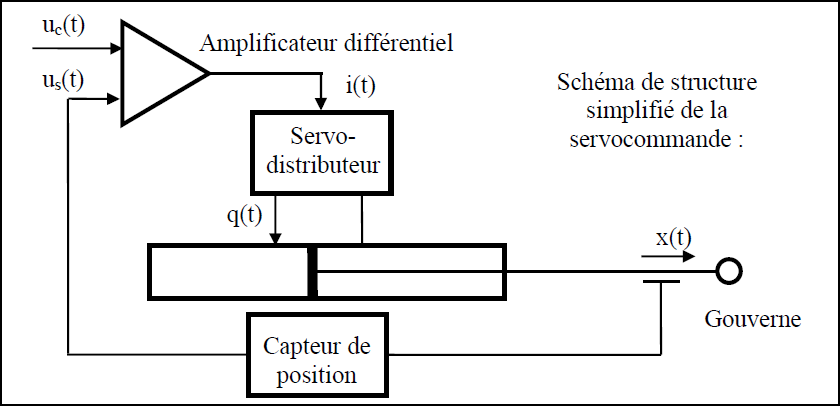
\includegraphics[width=\linewidth]{52_01}
\end{marginfigure}

Les différentes équations temporelles qui modélisent le fonctionnement d'une servocommande sont :
\begin{itemize}
\item un amplificateur différentiel défini par : $u_c(t)=\dfrac{i(t)}{K_a}+u_s(t)$;
\item débit dans le vérin dans le cas d'une hypothèse de fluide incompressible $q(t)=S\cdot\dfrac{\dd x(t)}{\dd t}$;
\item capteur de position : $u_s(t)=K_c\cdot x(t)$;
\item le servo-distributeur est un composant de la chaîne de commande conçu pour fournir un débit hydraulique $q(t)$ proportionnel au courant de commande $i(t)$. (Attention, valable uniquement en régime permanent.) On a 
$q(t)+T \dfrac{\dd q(t)}{\dd t} = K_d i(t)$.
%Le constructeur fournit sa fonction de transfert :
%$$
%F(p)=\dfrac{Q(p)}{I(p)}=\dfrac{K_d}{1+Tp}
%$$
%où $K_d$ est le gain du servo-distributeur et $T$ sa constante de temps.
\end{itemize}
 \fi
 
\question{Réaliser le schéma-blocs.}

\ifprof
On a :
\begin{itemize}
\item $U_c(p)=\dfrac{1}{K_a}I(p)+U_s(p)$
\item $Q(p)=SpX(p)$
\item $U_S(p)=K_C\cdot X(p)$
\item $F(p)=\dfrac{Q(p)}{I(p)}=\dfrac{K_d}{1+Tp}$
\end{itemize}

%\begin{minipage}[c]{.23\linewidth}
%\begin{marginfigure}
%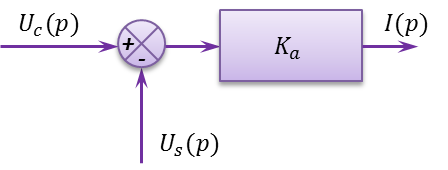
\includegraphics[width=.95\textwidth]{bloc1}
%\end{marginfigure}
%\end{minipage}\hfill
%\begin{minipage}[c]{.23\linewidth}
%\begin{marginfigure}
%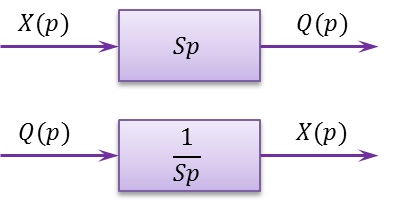
\includegraphics[width=.95\textwidth]{bloc2}
%\end{marginfigure}
%\end{minipage}\hfill
%\begin{minipage}[c]{.23\linewidth}
%\begin{marginfigure}
%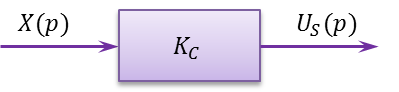
\includegraphics[width=.95\textwidth]{bloc3}
%\end{marginfigure}
%\end{minipage}\hfill
%\begin{minipage}[c]{.23\linewidth}
%\begin{marginfigure}
%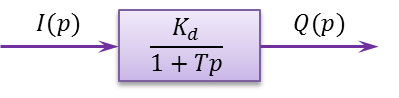
\includegraphics[width=.95\textwidth]{bloc4}
%\end{marginfigure}
%\end{minipage}

\begin{marginfigure}
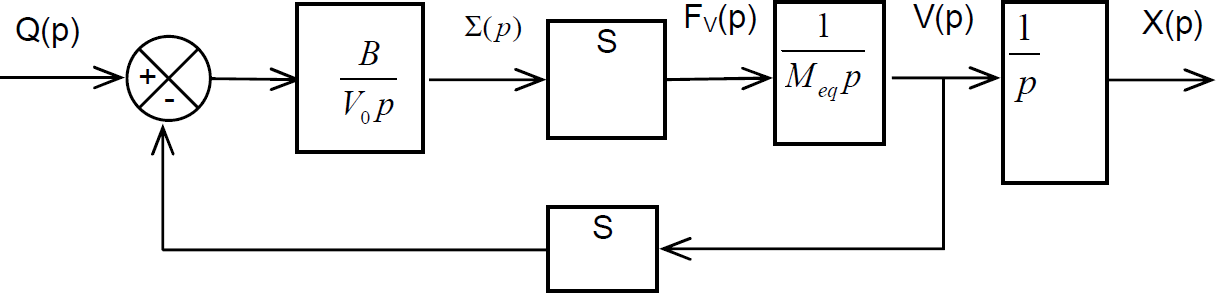
\includegraphics[width=\linewidth]{cor_01}
\end{marginfigure}

\else 
\fi


%\question{Réaliser le schéma-blocs.}
%\ifprof
%\begin{marginfigure}
%\centering
%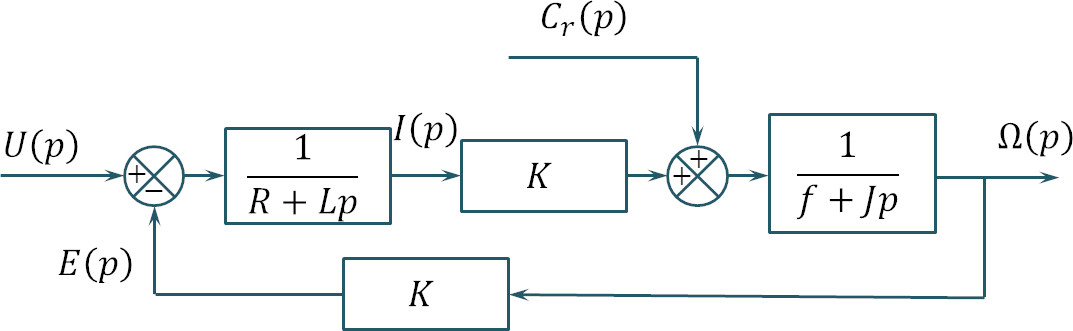
\includegraphics[width=\linewidth]{51_01_c}
%%\caption{Évolution du couple utile en fonction de la vitesse de rotation pour des
%%fréquences de commande de \SI{90}{Hz} à \SI{110}{Hz}. \label{fig_50_04}}
%\end{marginfigure}
%\else
%\fi


 

\ifprof
\else

\marginnote{Corrigé voir \ref{B2:07:52}.}

\fi